% fig14_theta_form.tex — theta division-vs-multiplication bug, charted.
% Compiled by the paper Makefile via `make figures` (pdflatex on the snippet).
%
% Data provenance (NO fabrication; commons @D g3) — Appendix B (app:bh-eq), the
% "theta-as-divisor trap" war story. Bosch-Hale Eq.(theta) writes the rational
% correction as the DIVISOR of T:  theta = T / [1 - T(...)/(1+T(...))].
%   The first porting mis-transcribed it as a MULTIPLICATION
%     theta = T * [1 - T(...)/(1+T(...))], which produced a uniform ~4x LOW
%     reactivity at EVERY temperature (the suspiciously clean factor of 4 sent
%     the chase after a phantom 4 pi; the actual cause was the textual
%     division-vs-multiplication typo).
%   Charted as the reactivity ratio to the correct (division) form:
%     division form (correct)    = 1.0x  (matches Bosch-Hale Table VIII, |d|=0)
%     multiplication form (bug)  ~ 0.25x (the ~4x-low artifact)
%   The "purely textual" pitfall: identical symbols, division vs multiplication.
%
% Manual single-shot compile (debug):
%   pdflatex -interaction=nonstopmode -halt-on-error fig14_theta_form.tex
\documentclass[border=4pt]{standalone}
\usepackage{tikz}
\usepackage{pgfplots}
\pgfplotsset{compat=1.18}
\begin{document}
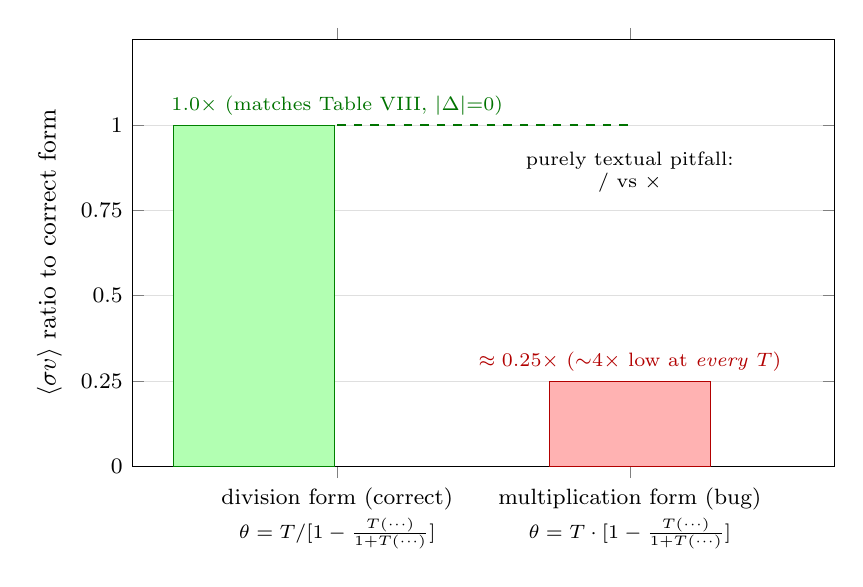
\begin{tikzpicture}
\begin{axis}[
  width=10.5cm, height=7cm,
  ybar,
  bar width=58pt,
  ymin=0, ymax=1.25,
  ytick={0,0.25,0.5,0.75,1.0},
  ylabel={$\langle\sigma v\rangle$ ratio to correct form},
  symbolic x coords={division, mult},
  xtick={division, mult},
  xticklabels={%
    \shortstack{division form (correct)\\\scriptsize $\theta=T/[1-\frac{T(\cdots)}{1+T(\cdots)}]$},
    \shortstack{multiplication form (bug)\\\scriptsize $\theta=T\cdot[1-\frac{T(\cdots)}{1+T(\cdots)}]$}},
  x tick label style={font=\footnotesize,align=center},
  tick label style={font=\footnotesize},
  label style={font=\small},
  ymajorgrids,
  grid style={gray!25},
  enlarge x limits=0.7,
  clip=false,
]
% correct (division) form = 1.0x, matches Table VIII
\addplot[draw=green!50!black,fill=green!30] coordinates {(division,1.0)};
% buggy (multiplication) form ~ 0.25x = 4x low at every T
\addplot[draw=red!70!black,fill=red!30,bar shift=0pt] coordinates {(mult,0.25)};
% reference line at 1.0 (correct = Table VIII)
\addplot[draw=green!45!black,dashed,thick,sharp plot,update limits=false] coordinates {
  (division,1.0) (mult,1.0)
};
% annotations
\node[font=\scriptsize,text=green!45!black,anchor=south] at (axis cs:division,1.0)
  {$1.0\times$ (matches Table VIII, $|\Delta|{=}0$)};
\node[font=\scriptsize,text=red!70!black,anchor=south] at (axis cs:mult,0.25)
  {$\approx0.25\times$ ($\sim$4$\times$ low at \emph{every} $T$)};
\node[font=\scriptsize,text=black,anchor=north,align=center]
  at (axis cs:mult,0.95)
  {purely textual pitfall:\\$/$ vs $\times$};
\end{axis}
\end{tikzpicture}
\end{document}
